\section{Classification}
\label{sec:modelSelection}
After the text data set, i.e., tweets are converted into numerical representation, remaining is the application of classification algorithms.
For this purpose, we employed several algorithms such as Logistic Regression, Naive Bayes, Random Forest (RF), Support Vector Machines (SVMs), Neural Networks (NNs) and Convolutional Neural Networks (CNNs).
After preliminary performance investigation of classification algorithms, we decided to continue our experiments with the three promising ones, which are explained below.
On the other hand, RF, which is really fast to compute, enabled us to evaluate the classification performance quickly for the first experiments.

\subsection{Support Vector Machines}
SVMs are very strong classification algorithms, even in high dimensional spaces, and the aim is to separate samples from different classes with a clear margin.
They can be applied as both linear binary classifiers and non-linear complements after kernel trick.
In our framework, we used the nonlinear SVM classifier implementation provided by \textit{scikit}\footnote{\url{http://scikit-learn.org/}}, which is a well-known, open-source machine learning library in Python.
After some experimentation, kernel function is chosen to be Radial Basis Function (RBF) and penalty parameter is used as $1$ for 10K iterations.


\subsection{Neural Networks}
NNs, as nonlinear function approximators trained via backpropagation, are configurable structures with number of layers, number of neurons per layers and nonlinearity options.
For our binary classification problem, we experimented with several network structures, some of which are presented in Section \ref{sec:results}.
Training is achieved using lbfgs algorithm, which is more memory friendly compared to SGD counterparts, with a constant learning rate of $10^{-5}$ for at most 1000 iteration, during which early stopping was possible when the cost function is noticed not to improve any more than $10^{-6}$.

\subsection{Convolutional Neural Networks}
\begin{figure}[h!]
	\centering
	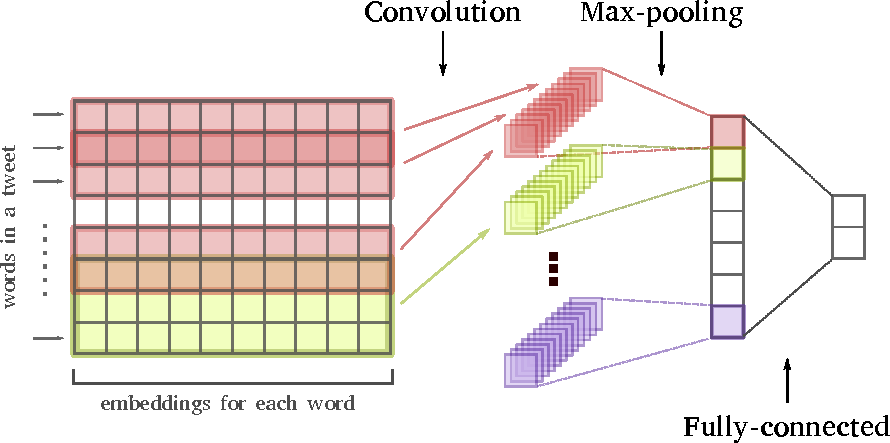
\includegraphics[width=0.8\columnwidth]{CNN_text.pdf}
	\caption{Convolutional Neural Networks for tweets}
	\label{fig:awesome_image}
\end{figure}

As well known for its success in computer vision area in the last years, CNNs are also applied to lots of NLP tasks with success \cite{kim14conv}. 
In order for CNN to be applied to text data, get trained by batches and understand the contextual relation between numerical representations of words, each tweet is assumed to be consisting of maximum number of words $n_{max}$ so that the each tweet is represented by a matrix with a size of $n_{max} \times D$, where $D$ represents the dimension of representation, which is GloVe vectors in our case.
Notice that all these matrices are zero-padded in the absence of words.
The main idea behind is to apply a bunch of filters with different window sizes to convolve, decrease the number of data by \textit{max-pooling} and apply \textit{soft max} layer as the classifier, which is illustrated in Figure \ref{fig:cnn}, where red filters have a window size of 2 and green ones 3, etc.
Although we experimented with different training strategies, the results to be presented in Section \ref{sec:results} are trained with minibatches of size 1024, Adam optimizer with a exponentially decaying learning rate every 1000 epoch, which is initialized as $5 \times 10^{-4}$. 
$n_{max}$ is chosen to be 40 for all the experiments.
Our CNN implementation relies on \textit{Tensorflow}\footnote{\url{https://www.tensorflow.org/}}, which is developed by Google and an open source software library for numerical computation using data flow graphs.